\subsection{Snailshell-Hypotrocoid profile of interpolated points}

\begin{table}[ht]
	\begin{center}
		\begin{tabular}[top]{ p{16.0 cm} }
			\frame{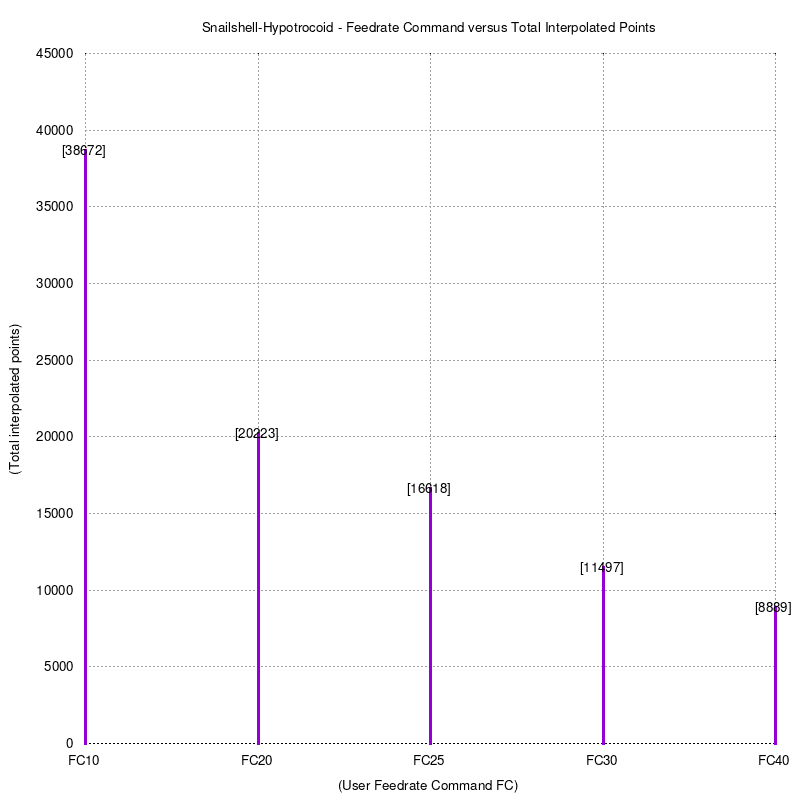
\includegraphics[width=0.95\textwidth]{./07-images/img-Ch51/Img-08-SnaHyp-Total-Interpolated-Points.png}}\\
		\end{tabular}
		\caption{SnaHyp profile of interpolated points}		
		\label{table:SnaHyp profile of interpolated points}
	\end{center}
\end{table} 
